\documentclass{beamer}


\usepackage[utf8]{inputenc}
\usepackage{amsmath}
\usepackage{amsfonts}
\usepackage{amssymb}
\usepackage{graphicx}
\usepackage{ragged2e}  % `\justifying` text
\usepackage{booktabs}  % Tables
\usepackage{tabularx}
\usepackage{tikz}      % Diagrams
\usetikzlibrary{calc, shapes, backgrounds}
\usepackage{amsmath}
\usepackage{amssymb}
\usepackage{dsfont}
\usepackage{url}       % `\url
\usepackage{listings}  % Code listings
\usepackage[T1]{fontenc}


\usepackage{theme/beamerthemehbrs}

\author[]{Abhishek Padalkar}

\title{Dynamic Motion Primitives}
\subtitle{Research and Development Project}
\institute[HBRS]{Hochschule Bonn-Rhein-Sieg}
\date{\today}
\subject{Test beamer}

% \thirdpartylogo{path/to/your/image}


\begin{document}
	{
	\begin{frame}
	\titlepage
	\end{frame}
	}
	
	\begin{frame}{Introduction}
		\begin{itemize}
			\item Need for motion planning and motion policies
			\item Learning a motion from demonstration (\textit{LfD})
			\item Dynamic Motion Primitives
		\end{itemize}
	\end{frame}
	
	
	\begin{frame}{Formulation of DMP}
		\begin{equation}\label{DMP_1}
		\tau\dot{z} = \alpha_{z}(\beta_{z}(g - y) - z) + f(x)
		\end{equation}
		\begin{equation}\label{DMP_2}
		\tau \dot{y} = z
		\end{equation}
		\begin{equation}\label{forcing_term}
		f(x) = \frac{\sum_{i=1}^{N}\psi_{i}(x)w_{i}}{\sum_{i=1}^{N}\psi_{i}(x)}x(g - y_{0})
		\end{equation}
		where,
		\begin{equation}\label{psi}
		\psi_{i} = \exp(-{\frac{1}{2\sigma_{i}^{2}}(x - c_{i})^{2}})
		\end{equation}
		and,
		\begin{equation}\label{canonical}
		\tau \dot{x} = -\alpha_{x}x
		\end{equation}
	\end{frame}
	
	\begin{frame}{Working of DMP}
		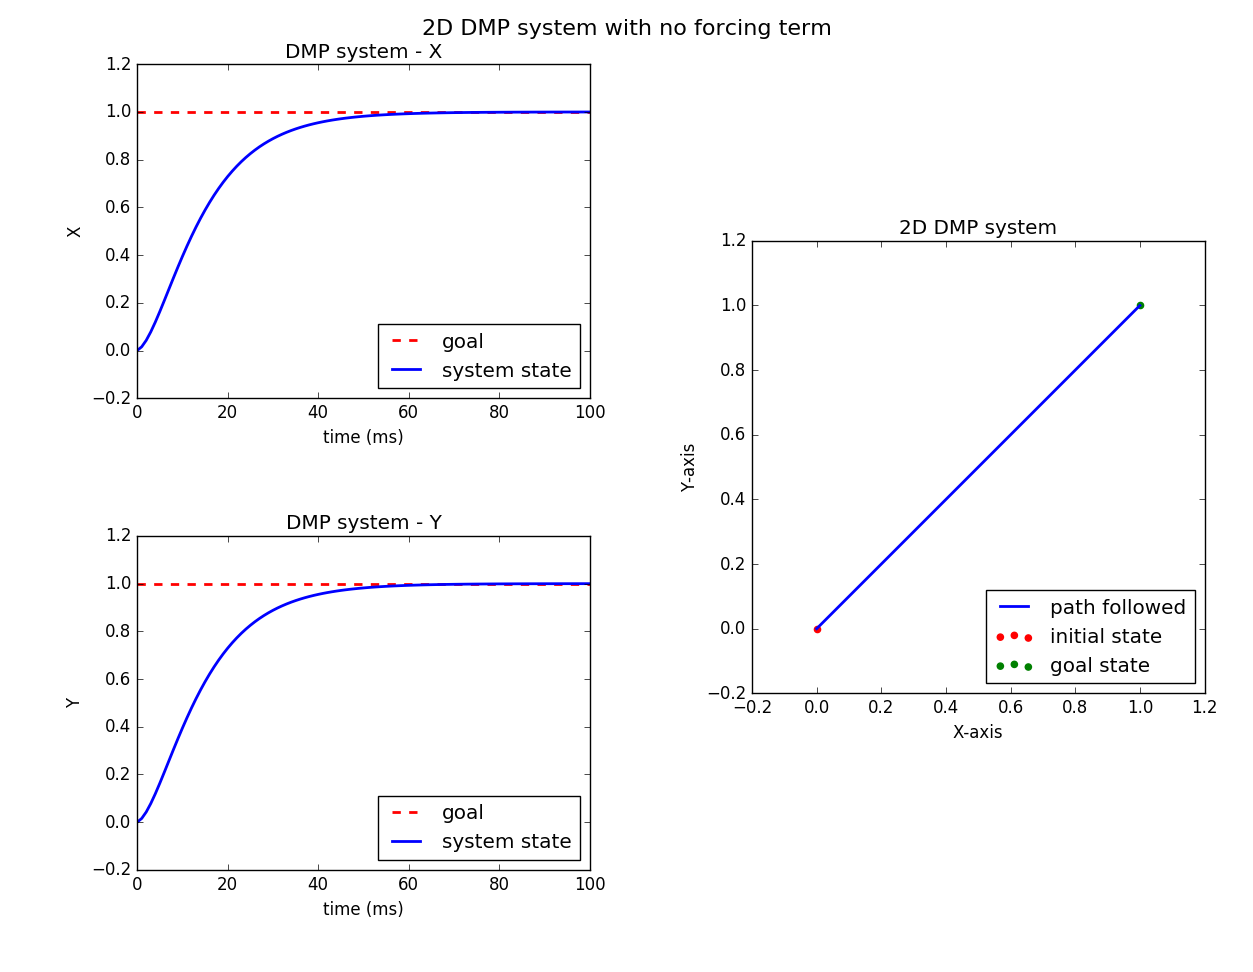
\includegraphics[width=\textwidth]{images/dmp_no_f}
	\end{frame}
	\begin{frame}
		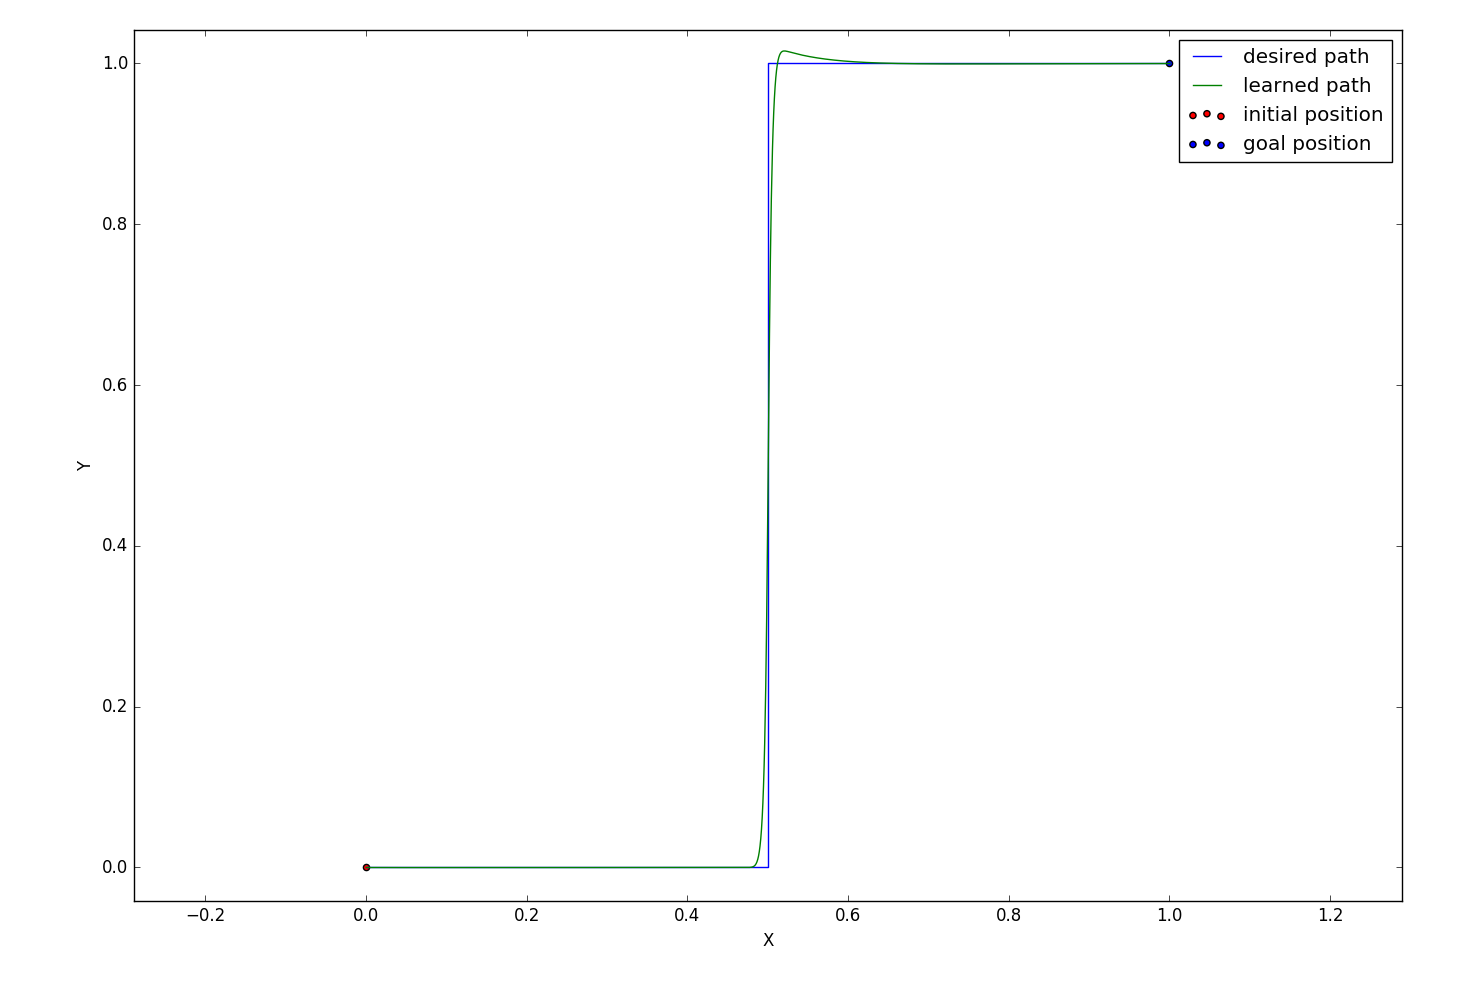
\includegraphics[width=\textwidth]{images/step_f}
	\end{frame}
	\begin{frame}
		\begin{figure}
			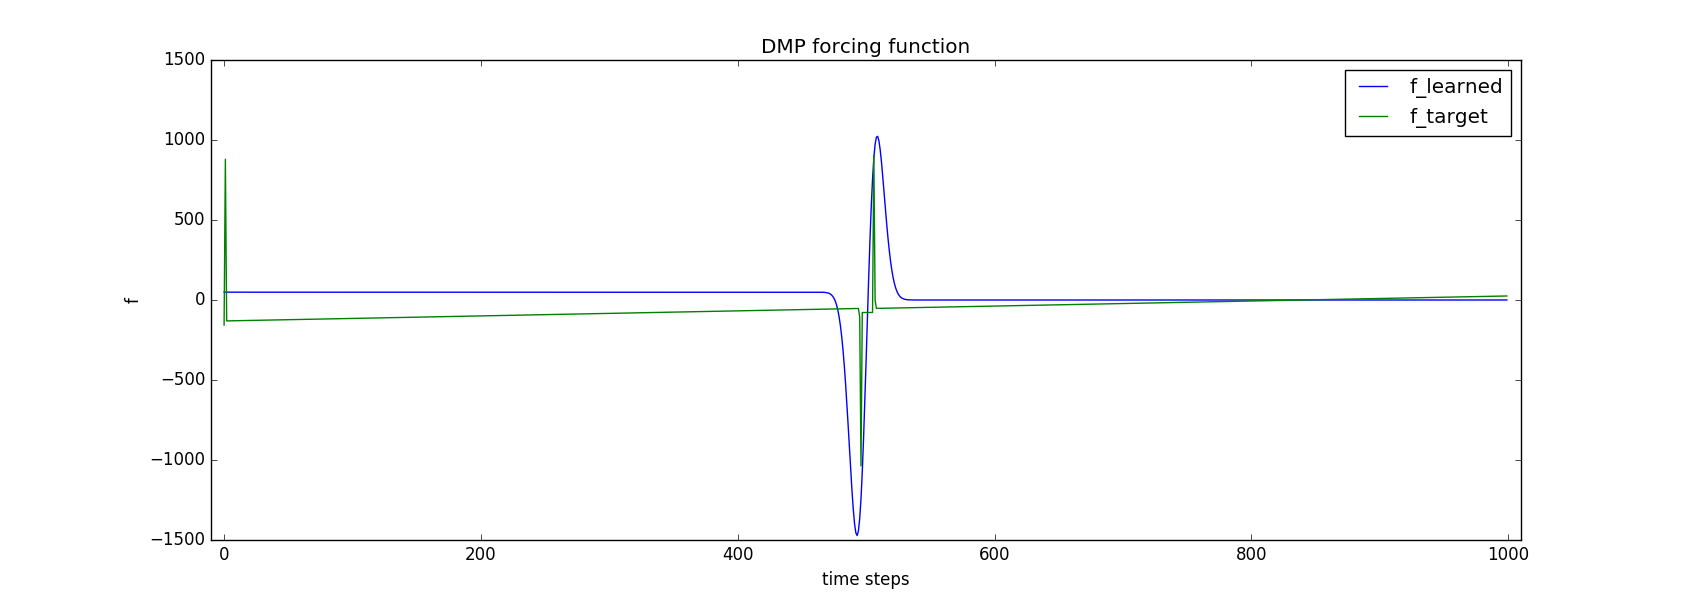
\includegraphics[scale=0.23]{images/f_x}
			\caption{Forcing term - X}
		\end{figure}

		\begin{figure}
			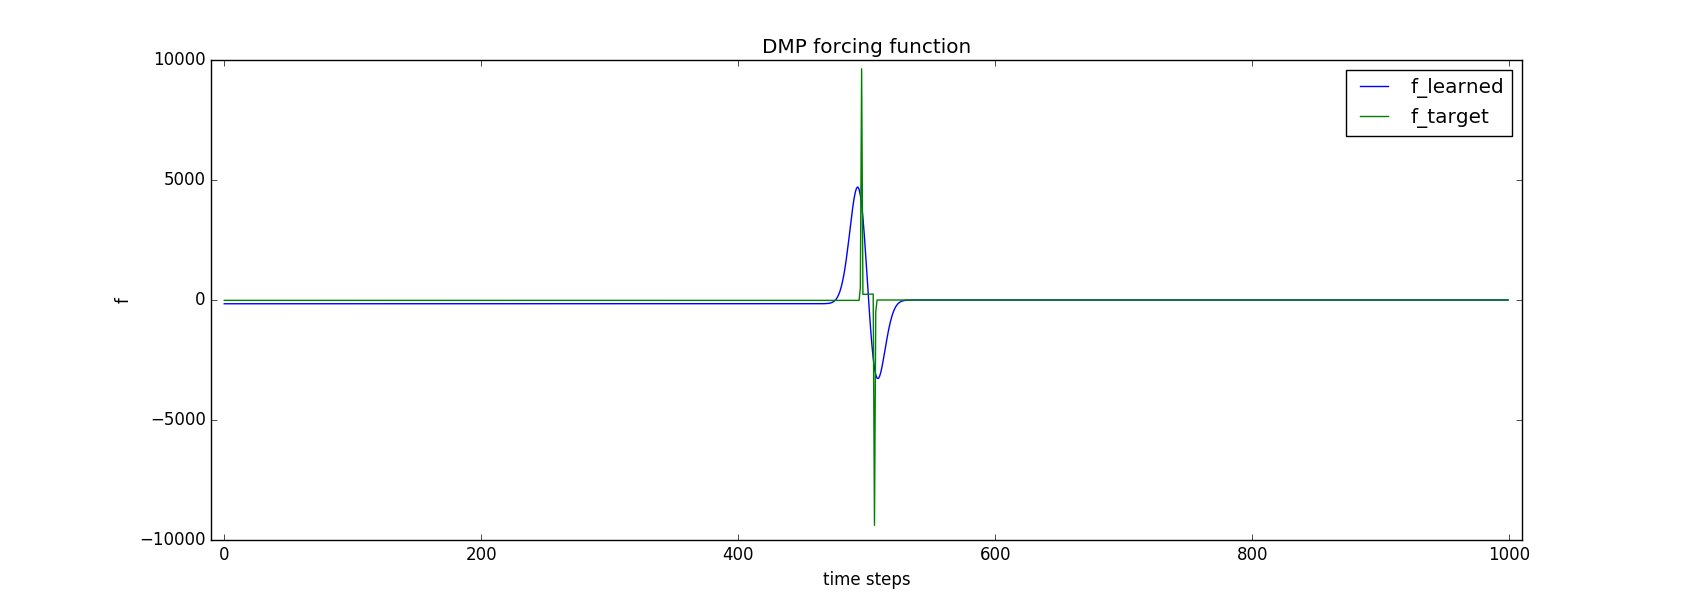
\includegraphics[scale=0.23]{images/f_y}
			\caption{Forcing term - Y}
		\end{figure}

	\end{frame}
	
	\begin{frame}{Analysis of the effects of the parameters used in DMP}
	
	\end{frame}
	
	\begin{frame}{Inverse Kinematic Solver}
		
	\end{frame}
	
	\begin{frame}{Whole Body Motion Control}
	
	\end{frame}
	
	\begin{frame}{Results}
	
	\end{frame}
	
	\begin{frame}{Conclusion}
	
	\end{frame}

\end{document}
